In the preliminaries we have seen how parity games can be used to verify if a modal $\mu$-calculus formula is satisfied by an LTS. Such a parity game contains the information needed to answer the question if an LTS satisfies a  modal $\mu$-calculus formula. We have also seen how an LTS can be extended with transition guards to model the behaviour of multiple LTSs. In this section we introduce \textit{variability parity games} (VPGs); a VPG extends the definition of a parity game much like an FTS extends the definition of an LTS. Similar as to how an FTS expresses multiple LTSs does a VPG express multiple parity games, moreover we introduce a way of creating VPGs such that every parity game it expresses contains the information needed to answer the question if a product in an FTS satisfies a modal $\mu$-calculus formula.

We extend parity games such that edges in the game are guarded. Instead of using features, feature expressions and products we choose a syntactically simpler representation and introduce the \textit{configurations}. A VPG has a set of configurations, the VPG can be played for a single configuration. Edges are guarded by sets of configurations; if the VPG is played for a configuration that is in the guard set then the edge is enabled, otherwise it is disabled.

\begin{definition}
	\label{def_VPG}
	A variability parity game (VPG) is a tuple $(V,V_0, V_1, E, \Omega, \mathfrak{C}, \theta)$, where:
	\begin{itemize}
		\item $V$,$V_0$,$V_1$, $E$ and $\Omega$ are defined as in parity games,
		\item $\mathfrak{C}$ is a non-empty finite set of configurations,
		\item $\theta : E \rightarrow 2^\mathfrak{C}\ \backslash\ \emptyset$ is a total function mapping every edge to a set of configurations guarding that edge.
	\end{itemize}
\end{definition}
We only consider total VPGs, meaning that every vertex has at least one outgoing edge. Since edges are guarded with sets of configurations we also require that for every configuration $c \in \mathfrak{C}$ every vertex has at least one outgoing edge that admits configuration $c$, formally we have for all $v \in V$:
\[ \bigcup\{\theta(v,w)\ |\ (v,w) \in E\} = \mathfrak{C} \]









Before we can define variability parity games we first define \textit{featured parity games} (FPG), featured parity games extend the definition of parity games to capture the variability represented in an FTS. It uses the same concepts as FTSs: features, products and a function that guards edges. In this section we will introduce the definition of FPGs and show that solving them answers the verification questions for FTS: For which products in the FTS does its projection satisfy $\varphi$?

First we introduce the definition of an FPG:
\begin{definition}
	\label{def_FPG}
	A featured parity game (FPG) is a tuple $(V,V_0, V_1, E, \Omega, N, P, \gamma)$, where:
	\begin{itemize}
		\item $V = V_0 \cup V_1$ and $V_0 \cap V_1 = \emptyset$,
		\item $V_0$ is the set of vertices owned by player $0$,
		\item $V_1$ is the set of vertices owned by player $1$, 
		\item $E \subseteq V \times V$ is the edge relation,
		\item $\Omega :  V \rightarrow \mathbb{N}$ is a priority assignment,
		\item $N$ is a non-empty set of features,
		\item $P \subseteq \mathcal{P}(N)$ is a non-empty set of products, ie. feature assignments, for which the game can be played,
		\item $\gamma : E \rightarrow \mathbb{B}(N)$ is a total function, labelling each edge with a Boolean expression over the features.
	\end{itemize}
\end{definition}
An FPG is played similarly to a PG, however the game is played for a specific product $p \in P$. Player $\alpha$ can only move the token from $v \in V_\alpha$ to $w \in V$ if $(v,w) \in E$ and $p \models \gamma(v,w)$.

A game played for product $p \in P$ results in winnings sets $W_0^p$ and $W_1^p$, which are defined similar to the $W_0$ and $W_1$ winning sets for parity games.

An FPG can simply be projected to a product $p$ by removing the edges that are not satisfied by $p$.
\begin{definition}
	\label{def_FPG_proj}
	The projection from FPG $G = (V,V_0, V_1, E, \Omega, N, P, \gamma)$ to a product $p \in P$, noted $G_{|p}$, is the parity game $(V,V_0,V_1, E', \Omega)$ where $E' = \{ e \in E\ |\ p \models \gamma(e) \}$.
\end{definition}

Playing FPG $G$ for a specific product $p\in P$ is the same as playing the PG $G_{|p}$. Any path that is valid in $G$ for $p$ is also valid in $G_{|p}$ and vice versa. Therefore the strategies are also interchangeable, furthermore the winning sets $W_\alpha$ for $G_{|p}$ and $W_\alpha^p$ for $G$ are identical. Since parity games are positionally determined so are FPGs. Similarly, since finite parity games are decidable, so are finite FPGs.

We say that an FPG is solved when the winning sets for every valid product in the FPG are determined.
\subsubsection{Creating featured parity games}
An FPG can be created from an FTS in combination with a model $\mu$-calculus formula. We translate an FTS to an FPG by first creating a PG from the transition system as if there were no transition guards, next we apply the same guards to the FPG as are present in the FTS for edges that originate from transitions. The features and valid products in the FPG are identical to those in the FTS.
\begin{definition}
	\label{def_FTS2FPG}
	$FTS2FPG(M, \varphi)$ converts FTS $M = (S, Act, trans, s_0, N, P, \gamma)$ and closed formula $\varphi$ to FPG $(V, V_0, V_1, E, \Omega, N, P, \gamma')$.
	
	We have $(V, V_0, V_1, E, \Omega) = \textit{LTS2PG}((S, Act, trans, s_0), \varphi$) and
	\[ \gamma'((s, \psi),(s', \psi')) = \begin{cases}
	\gamma(s,a,s') & \text{if }\psi = \langle a \rangle \psi'\text{ or }\psi = [a]\psi' \\
	\top & \text{otherwise}
	\end{cases}\]
\end{definition}
Consider our working example which we extend to an FTS depicted in figure \ref{fig:exverfts}, for this example we have features $N = \{f, g\}$ and products $P = \{\emptyset, \{f\},\{f,g\}\}$.
\begin{figure}[h]
	\centering
	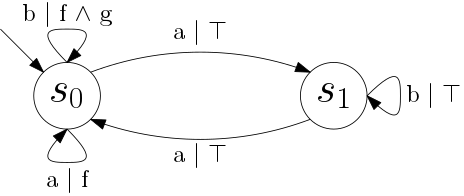
\includegraphics[scale=0.3]{Examples/ExamleVerification/FTS}
	\caption[FTS $M$]{FTS $M$}
	\label{fig:exverfts}
\end{figure}
\begin{figure}[h]
	\centering
	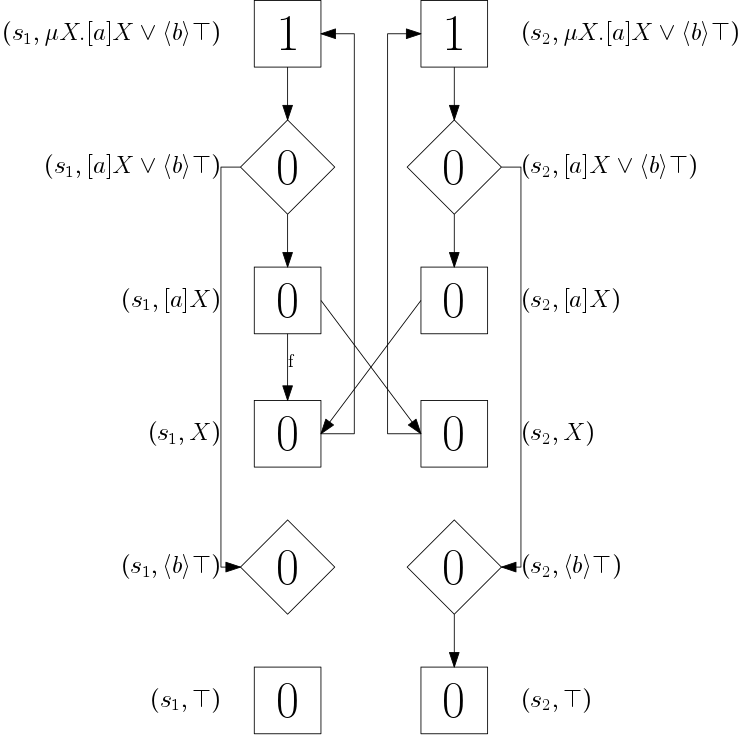
\includegraphics[scale=0.3]{Examples/ExamleVerification/FPG}
	\caption[FPG for $M$ and $\varphi$]{FPG for $M$ and $\varphi$}
	\label{fig:exverfpg}
\end{figure}
We can translate this FTS with formula $\varphi = \mu X. ([a] X \vee \langle b \rangle \top)$ to an FPG depicted in figure \ref{fig:exverfpg}. As we can see from the FTS if feature $f$ is enabled and $g$ is disabled then we have an infinite path of $a$'s where $b$ is never enabled, therefore $\varphi$ doesn't hold for $M_{|\{f\}}$. If $g$ is enabled however we can always do a $b$ so $\varphi$ holds for $M_{|\{f,g\}}$. As we have seen $\varphi$ does hold for $M_{|\emptyset}$. For the product $\emptyset$ we have the same winning set as before:
\begin{align*}
W_0^\emptyset = \{& (s_1, \mu X.\phi),\\
& (s_1, [a](\mu X.\phi) \vee \langle b \rangle \top),\\
& (s_1, [a](\mu X.\phi)),\\
& (s_1, \top),\\
& (s_2, \mu X.\phi),\\
& (s_2, [a](\mu X.\phi) \vee \langle b \rangle \top),\\
& (s_2, [a](\mu X.\phi)),\\
& (s_2, \langle b \rangle \top),\\
& (s_2, \top)
\}\\
W_1^\emptyset = \{& (s_1, \langle b \rangle \top )\}
\end{align*}
In the FPG we can see that if $f$ is enabled and $g$ is disabled then player $1$ can move the token from $(s_1, [a]X)$ to $(s_1,X)$. This results in player $0$ either moving the token to $(s_1, \langle b \rangle \top)$ and losing or an infinite path where $1$ occurs infinitely often which is also player $1$ wins. For product $\{f\}$ we have winning sets:
\begin{align*}
W_0^{\{f\}} = \{
& (s_1, \top),\\
& (s_2, \mu X.\phi),\\
& (s_2, [a](\mu X.\phi) \vee \langle b \rangle \top),\\
& (s_2, \langle b \rangle \top),\\
& (s_2, \top)
\}\\
W_1^{\{f\}} = \{& (s_1, \mu X.\phi),\\
& (s_1, [a](\mu X.\phi) \vee \langle b \rangle \top),\\
& (s_1, [a](\mu X.\phi)),\\
& (s_1, \langle b \rangle \top ),\\
& (s_2, [a](\mu X.\phi))\}
\end{align*}
However if $g$ is also enabled then player $0$ wins in $(s_1, \langle b \rangle \top)$, thus giving the following winning sets:
\begin{align*}
W_0^{\{f,g\}} = \{& (s_1, \mu X.\phi),\\
& (s_1, [a](\mu X.\phi) \vee \langle b \rangle \top),\\
& (s_1, [a](\mu X.\phi)),\\
& (s_1, \langle b \rangle \top ),\\
& (s_1, \top),\\
& (s_2, \mu X.\phi),\\
& (s_2, [a](\mu X.\phi) \vee \langle b \rangle \top),\\
& (s_2, [a](\mu X.\phi)),\\
& (s_2, \langle b \rangle \top),\\
& (s_2, \top)
\}\\
W_1^{\{f,g\}} = \{\}
\end{align*}

In the next section we will show how the winning sets relate to the model verification question.


\subsubsection{FTS verification using featured parity games}
We can create an FPG from an FTS and project it to a product, resulting in a PG, this is shown in the following diagram:\\
\begin{tikzpicture}
\matrix (m) [matrix of math nodes,row sep=4em,column sep=4em,minimum width=2em]
{
	\text{FTS} & \text{FPG} \\
	\  & \text{PG} \\};
\path[-stealth]
(m-1-1)
edge node [above] {$\varphi$} (m-1-2)

(m-1-2) edge [double] node [right] {$\Pi$} (m-2-2)
;
\end{tikzpicture}\\
Earlier we saw that we could also derive a PG by projecting the FTS to a product and then translation the resulting LTS to a PG, depicted by the following diagram:
\\\begin{tikzpicture}
\matrix (m) [matrix of math nodes,row sep=4em,column sep=4em,minimum width=2em]
{
	\text{FTS} \\
	\text{LTS} & \text{PG} \\};
\path[-stealth]
(m-1-1) edge [double] node [left] {$\Pi$} (m-2-1)
(m-2-1.east|-m-2-2) edge node [above] {$\varphi$}
(m-2-2)
;
\end{tikzpicture}\\
We will now show that the resulting parity games are identical.
\begin{theorem}
	\label{the_PGsubPGA} Given:
	\begin{itemize}
		\item FTS $M = (S,Act, trans, s_0, N, P, \gamma)$,
		\item a closed modal mu-calculus formula $\varphi$,
		\item a product $p \in P$
	\end{itemize}
	it holds that the parity games LTS2PG($M_{|p}, \varphi$) and FTS2FPG($M, \varphi$)$_{|p}$  are identical.
	\begin{proof}
		Let $G^F = (V^F, V_0^F, V_1^F, E^F, \Omega^F, N, P, \gamma') = FTS2FPG(M, \varphi)$, using definition \ref{def_FTS2FPG}, and $G^F_{|p} = (V^F, V_0^F, V_1^F, {E^F}', \Omega^F)$, using definition \ref{def_FPG_proj}. Furthermore we have $M_{|p} = (S, Act, trans', s_0)$ and we let $G = (V, V_0, V_1, E, \Omega) =  LTS2PG(M_{|p}, \varphi)$. We depict the different transition systems and games in the following diagram.
		
		\begin{tikzpicture}
		\matrix (m) [matrix of math nodes,row sep=4em,column sep=1em,minimum width=2em]
		{
			\text{\ \ FTS }M & \  &\ & \text{FPG } G^F  \\
			\text{LTS }M_{|p} & \ & \text{PG } G & \text{\ \ PG }G_{|p}^F \\};
		\path[-stealth]
		(m-1-1) edge [double] node [left] {$\Pi$} (m-2-1)
		edge node [above] {$\varphi$} (m-1-4)
		(m-2-1.east|-m-2-3) edge node [above] {$\varphi$}
		(m-2-3)
		(m-1-4) edge [double] node [right] {$\Pi$} (m-2-4);
		\end{tikzpicture}\\
		We will prove that $G = G_{|p}^F$. We first note that game $G$ is created by 
		\[  (V, V_0, V_1, E, \Omega) = LTS2PG((S, Act, trans', s_0),\varphi) \]
		and the vertices, edges and priorities of game $G^F$ are created by 
		\[ (V^F, V_0^F, V_1^F, E^F, \Omega^F) = LTS2PG((S,Act, trans, s_0), \varphi)\]
		Using the definition of LTS2PG (\ref{def_LTS2PG}) we find that the vertices and the priorities only depend on the states in $S$ and the formula $\varphi$, since these are identical in the above two statements we immediately get $V = V^F, V_0 = V_0^F, V_1 = V_1^F$ and $\Omega = \Omega^F$. The vertices and priorities don't change when an FTS is projected, therefore $G_{|p}^F$ has the same vertices and priorities as $G^F$.
		
		Now we are left with showing that $E = {E^F}'$ in order to conclude that that $G = G^F_{|p}$. We will do this by showing $E \subseteq {E^F}'$ and $E \supseteq {E^F}'$.
		
		First let $e \in E$. Note that a vertex in the parity game is represented by a pair of a state and a formula. So we can write $e = ((s,\psi),(s',\psi'))$. To show that $e \in {E^F}'$ we distinguish two cases:
		\begin{itemize}
			\item  If $\psi = \langle a \rangle \psi'$ or $\psi = [a] \psi'$ then there exists an $a \in Act$ such that $(s,a,s') \in trans'$. Using the FTS projection definition (\ref{def_fts_proj}) we get $(s,a,s') \in trans$ and $p \models \gamma(s,a,s')$. Using the FTS2FPG definition (\ref{def_FTS2FPG}) we find that $\gamma'((s,\psi),(s',\psi')) = \gamma(s,a,s')$ and therefore $p \models \gamma'((s,\psi),(s',\psi'))$. Now using the FPG projection definition (\ref{def_FPG_proj}) we find $((s,\psi),(s',\psi')) \in {E^F}'$.
			\item Otherwise the existence of the edge does not depend on the $trans$ parameter and therefore $((s,\psi),(s',\psi')) \in {E^F}'$ if $(s,\psi) \in V^F$, since $V^F = V$ we have $(s,\psi) \in V^F$.
		\end{itemize}
		We can conclude that $E \subseteq {E^F}'$, next we will show $E \supseteq {E^F}'$. Let $e = ((s,\psi),(s',\psi')) \in {E^F}'$. We distinguish two cases:
		\begin{itemize}
			\item If $\psi = \langle a \rangle \psi'$ or $\psi = [a] \psi'$ then there exists an $a \in Act$ such that $(s,a,s') \in trans$. Using the FPG projection definition (\ref{def_FPG_proj}) we get $p \models \gamma'(s,a,s')$. Using the FTS2FPG definition (\ref{def_FTS2FPG}) we get $p \models \gamma(s,a,s')$. Using the FTS projection definition (\ref{def_fts_proj}) we get $(s,a,s') \in trans'$ and therefore $((s,\psi),(s',\psi'))\in E$.
			\item Otherwise the existence of the edge does not depend on the $trans$ parameter and therefore $((s,\psi),(s',\psi')) \in E$ if $(s,\psi) \in V$, since $V^F = V$ we have $(s,\psi) \in V$.
		\end{itemize}
	\end{proof}
\end{theorem}

Having proven this we can visualize the relation between the different games and transition systems in the following diagram:
\\\begin{tikzpicture}
\matrix (m) [matrix of math nodes,row sep=4em,column sep=4em,minimum width=2em]
{
	\text{FTS} & \text{FPG} \\
	\text{LTS} & \text{PG} \\};
\path[-stealth]
(m-1-1) edge [double] node [left] {$\Pi$} (m-2-1)
edge node [above] {$\varphi$} (m-1-2)
(m-2-1.east|-m-2-2) edge node [above] {$\varphi$}
(m-2-2)
(m-1-2) edge [double] node [right] {$\Pi$} (m-2-2)
;
\end{tikzpicture}\\
Finally we prove that solving an FTS, ie. finding winning sets for all products, answers the verification question.
\begin{theorem}
	\label{the_FPG_ver_FTS}
	Given:
	\begin{itemize}
		\item FTS $M = (S, Act, trans, s_0, N, P, \gamma)$,
		\item closed modal mu-calculus formula $\varphi$,
		\item product $p \in P$ and
		\item state $s \in S$
	\end{itemize}
	it holds that $(M_{|p}, s) \models \varphi$ if and only if $(s, \varphi) \in W_0^p$ in $\textit{FTS2FPG}(M, \varphi$).
	\begin{proof}
		The winning set $W_\alpha^p$ is equal to winning set $W_\alpha$ in $\textit{FTS2FPG}(M, \varphi)_{|p}$, for any $\alpha \in \{0,1\}$, using the FPG definition (\ref{def_FPG}). Using theorem \ref{the_PGsubPGA} we find that the game $FTS2FPG(M, \varphi)_{|p}$ is equal to the game $LTS2PG(M_{|p}, \varphi)$, obviously their winning sets are also equal. Using the well studied relation between parity games and LTS verification, stated in theorem \ref{the_LTS_PG_REL}, we know that $(M_{|p}, s) \models \varphi$ if and only if $(s, \varphi) \in W_0$ in game $LTS2PG(M_{|p},\varphi)$. Winning set $W_\alpha^p$ is equal to $W_\alpha$, therefore the theorem holds.
	\end{proof}
\end{theorem}

Revisiting our prior example we can see the theorem in action by noting that $M_{|\emptyset} \models \varphi$ , $M_{|\{f\}} \not\models \varphi$ and $M_{|\{f,g\}} \models \varphi$. This is reflected by the vertex $(s_1, \mu X. [a]X \vee \langle b \rangle \top)$ being present in $W_0^\emptyset$ and $W_0^{\{f,g\}}$ but not in $W_0^{\{f\}}$.

\subsection{Variability parity games}
Next we will introduce \textit{variability parity games} (VPGs). VPGs are very similar to FPGs, however VPGs use configurations instead of features and products to express variability. This gives a syntactically more pleasant representation that is not solely tailored for FTSs. Furthermore in VPGs deadlocks are removed, by doing so VPG plays can only result in infinite paths and no longer in finite paths.

Later we will show the relation between VPGs and FTS verification, which is similar to the relation between FPGs and FTS verification. First we introduce VPGs.

A VPG is played similarly to a PG, however the game is played for a specific configuration $c \in \mathfrak{C}$. Player $\alpha$ can only move the token from $v \in V_\alpha$ to $w \in V$ if $(v,w) \in E$ and $c \in \theta(v,w)$. Furthermore VPGs don't have deadlocks, therefore every play results in an infinite path.

A game played for configuration $c \in \mathfrak{C}$ results in winning sets $W_0^c$ and $W_1^c$, which are defined similar to the $W_0$ and $W_1$ winning sets for parity games.

Solving a VPG means determining winning sets for every configuration in the VPG.
\begin{definition}
	\label{def_VPG_proj} The projection from VPG $G = (V, V_0, V_1, E, \Omega, \mathfrak{C}, \theta)$ to a configuration $c \in \mathfrak{C}$, noted $G_{|c}$, is the parity game $(V, V_0, V_1, E', \Omega)$ where $E' = \{ e\in E\ |\ c \in \theta(e)\}$.
\end{definition}

Playing VPG $G$ for a specific configuration $c \in \mathfrak{C}$ is the same as playing the PG $G_{|c}$. Any path that is valid in $G$ for $c$ is also valid in $G_{|c}$ and vice versa. Therefore the strategies are also interchangeable, furthermore the winning sets $W_\alpha$ for $G_{|c}$ and $W_\alpha^c$ for $G$ are identical. Since parity games are positionally determined so are VPGs. Similarly, since finite parity games are decidable, so are finite VPGs.
\subsubsection{Creating variability parity games}
We will define a translation from an FPG to a VPG. To do so we use the set of valid products as the set of configurations. Furthermore we make the FPG deadlock free, this is done by creating two losing vertices $l_0$ and $l_1$ such that player $\alpha$ loses when the token is in vertex $l_\alpha$. Any vertex that can't move for a configuration will get an edge that is admissible for that configuration towards one of the losing vertices.
\begin{definition}
	\label{def_FPG2VPG}
	FPG2VPG($G^F$) converts FPG $G^F = (V^F, V_0^F, V_1^F, E^F, \Omega^F, N, P, \gamma)$ to VPG $G = (V, V_0, V_1, E, \Omega, \mathfrak{C}, \theta)$.
	
	We define $\mathfrak{C} = P$. We create vertices $l_0$ and $l_1$ and define $V_0 = V_0^F \cup \{l_0\}$, $V_1 = V_1^F \cup \{l_1\}$ and $V = V_0 \cup V_1$.
	
	We construct $E$ by first making $E = E^F$ and adding edges $(l_0, l_0)$ and $(l_1, l_1)$ to $E$. Simultaneously we construct $\theta$ by first making $\theta(e) = \{p \in \mathfrak{C}\ |\ p \models \gamma(e)\}$ for every $e \in E^F$. Furthermore $\theta(l_0,l_0) = \theta(l_1,l_1) = \mathfrak{C}$.
	
	Next, for every vertex $v \in V_\alpha$ with $\alpha = \{0,1\}$, we have $C = \mathfrak{C} \backslash \bigcup \{\theta(v,w)\ |\ (v,w) \in E\}$. If $C \neq \emptyset$ then we add $(v, l_\alpha)$ to $E$ and make $\theta(v,l_\alpha) = C$.
	Finally we have 
	\[ \Omega(v) = \begin{cases}
	1  & \text{if } v = l_0 \\
	0 & \text{if } v = l_1 \\
	\Omega^F(v) &\text{otherwise}
	\end{cases} \]
\end{definition}
Again considering our previous working example we can translate the FPG shown in figure \ref{fig:exverfpg} to the VPG shown in figure \ref{fig:exvevpg}. Where $c_0$ is product $\emptyset$, $c_1$ is $\{f\}$ and $c_2$ is $\{f,g\}$.
\begin{figure}[h]
	\centering
	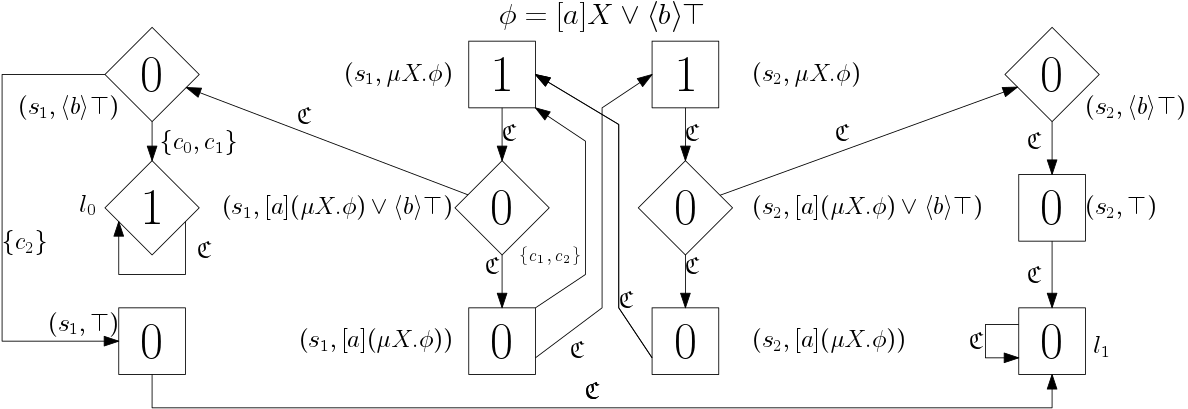
\includegraphics[scale=0.3]{Examples/ExamleVerification/VPG}
	\caption[VPG]{VPG}
	\label{fig:exvevpg}
\end{figure}

\subsubsection{FTS verification using variability parity games}
We have shown in theorem \ref{the_FPG_ver_FTS} that we can use an FPG to verify an FTS. Next we will show that a winning set in the FPG $M$ is the subset of the winning set in the VPG $\textit{FPG2VPG}(M)$.
\begin{theorem}
	\label{the_FPG_sub_VPG}
	Given:
	\begin{itemize}
		\item FPG $G^F = (V^F, V_0^F, V_1^F, E^F, \Omega^F, N, P, \gamma)$,
		\item product $p \in P$
	\end{itemize}
	we have for winning sets $Q_\alpha^{p}$ in $G^F$ and $W_\alpha^{p}$ in $\textit{FPG2VPG}(G^F)$ that $Q_\alpha^{p} \subseteq W_\alpha^{p}$ for any $\alpha \in \{0,1\}$.
	\begin{proof}
		Let $G = (V,V_0,V_1, E, \Omega, \mathfrak{C},\theta) = \textit{FPG2VPG}(G^F)$. Consider finite play $\pi$ that is valid in game $G^F$ for product $p$. We have for every $(\pi_i, \pi_{i+1})$ in $\pi$ that $(\pi_i, \pi_{i+1}) \in E^F$ and $p \models \gamma(\pi_i, \pi_{i+1})$. From the $\textit{FPG2VPG}$ definition (\ref{def_FPG2VPG}) it follows that $(\pi_i, \pi_{i+1}) \in E$ and $p \in \theta(\pi_i, \pi_{i+1})$. So we can conclude that path $\pi$ is also valid in game $G$ for configuration $p$. Since the play is finite the winner is determined by the last vertex $v$ in $\pi$, player $\alpha$ wins such that $v \in V_{\overline{\alpha}}$. Furthermore we know, because the play is finite, that there exists no $(v,w) \in E^F$ with $p \models \gamma(v,w)$. From this we can conclude that $(v, l_{\overline{\alpha}}) \in E$ and $p \in \theta(v, l_{\overline{\alpha}})$. Vertex $l_{\overline{\alpha}}$ has one outgoing edge, namely to itself. So finite play $\pi$ will in game $G^F$ results in an infinite play $\pi(l_{\overline{\alpha}})^\omega$. Vertex $l_{\overline{\alpha}}$ has a priority with the same parity as player $\alpha$, so player $\alpha$ wins the infinite play in $G$ for configuration $p$.
		
		Consider infinite play $\pi$ that is valid in game $G^F$ for product $p$. As shown above this play is also valid in game $G$ for configuration $p$. Since the win conditions of both games are the same the play will result in the same winner.
		
		Consider infinite play $\pi$ that is valid in game $G$ for configuration $p$. We distinguish two cases:
		\begin{itemize}
			\item If $l_\alpha$ doesn't occur in $\pi$ then the path is also valid for game $G^F$ with product $p$ and has the same winner.
			\item If $\pi = \pi'(l_\alpha)^\omega$ with no occurrence of $l_\alpha$ in $\pi'$ then the winner is player $\overline{\alpha}$. The path $\pi'$ is valid for game $G^F$ with product $p$. Let vertex $v$ be the last vertex of $\pi'$. Since $(v, l_\alpha) \in E$ and $p \in \theta(v,l_\alpha)$ we know that there is no $(v,w) \in E^F$ with $p \models \gamma(v,w)$ and that vertex $v$ is owned by player $\alpha$. So in game $G^F$ player $\alpha$ can't move at vertex $v$ and therefore loses the game (in which case the winner is also $\overline{\alpha}$).
		\end{itemize}
		
		We have shown that every path (finite or infinite) in game $G^F$ with product $p$ can be played in game $G$ with configuration $p$ and that they have the same winner. Furthermore every infinite path in game $G$ with configuration $p$ can be either played as an infinite path or the first part of the path can be played in $G^F$ with product $p$ and they have the same winner. From this we can conclude that the theorem holds.
	\end{proof}
\end{theorem}
We can conclude the diagram depicting the relation between the different games and transition systems:\\
\begin{tikzpicture}
\matrix (m) [matrix of math nodes,row sep=4em,column sep=4em,minimum width=2em]
{
	\text{FTS} & \text{FPG} & \text{VPG} \\
	\text{LTS} & \text{PG} \\};
\path[-stealth]
(m-1-1) edge [double] node [left] {$\Pi$} (m-2-1)
edge node [above] {$\varphi$} (m-1-2)
(m-2-1.east|-m-2-2) edge node [above] {$\varphi$}
(m-2-2)
(m-1-2) edge [double] node [right] {$\Pi$} (m-2-2)
edge (m-1-3);
\end{tikzpicture}\\
Finally we show that solving VPGs, ie. finding the winning sets for all configurations, can be used to verify FTSs.
\begin{theorem}
	\label{the_VPG_ver_FTS}
	Given:
	\begin{itemize}
		\item FTS $M = (S, Act, trans, s_0, N, P, \gamma)$,
		\item closed modal mu-calculus formula $\varphi$,
		\item product $p \in P$ and
		\item state $s \in S$
	\end{itemize}
	it holds that $(M_{|p}, s) \models \varphi$ if and only if $(s, \varphi) \in W_0^{p}$ in $\textit{FPG2VPG}(\textit{FTS2FPG}(M, \varphi))$.
	\begin{proof}
		Let $W_0^{p}$ and $W_1^{p}$ denote the winning sets for game $\textit{FPG2VPG}(\textit{FTS2FPG}(M, \varphi))$. And $Q_0^{p}$ and $Q_1^{p}$ denote the winning sets for game $\textit{FTS2FPG}(M, \varphi)$.
		
		Using theorem \ref{the_FPG_ver_FTS} we find that $(M_{|p}, s) \models \varphi$ if and only if $(s, \varphi) \in Q_0^{p}$. If $(s, \varphi) \in Q_0^{p}$ then we find by using theorem \ref{the_FPG_sub_VPG} that $(s, \varphi) \in W_0^{p}$. If $(s, \varphi) \not\in Q_0^{p}$ then $(s, \varphi) \in Q_1^{p}$ and therefore $(s, \varphi) \in W_1^{p}$ and $(s, \varphi) \not\in W_0^{p}$.
	\end{proof}
\end{theorem}
Using this theorem we can visualize verification of an FTS in figure \ref{fig:ftsverificationusingvpg}.
\begin{figure}[h]
	\centering
	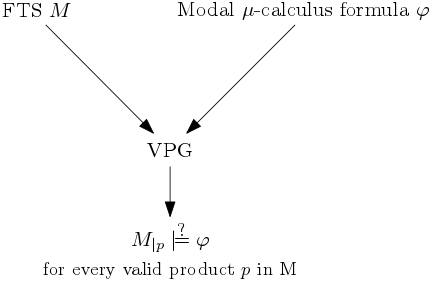
\includegraphics[scale=0.5]{Diagrams/FTSVerificationUsingVPG}
	\caption[FTS verification using VPG]{FTS verification using VPG}
	\label{fig:ftsverificationusingvpg}
\end{figure}

